\documentclass[a4paper,12pt]{jsarticle}

\usepackage{amsmath,amssymb}
\usepackage{bm}
\usepackage[dvipdfmx]{graphicx}
\usepackage{verbatim}
\usepackage{wrapfig}
\usepackage{ascmac}
\usepackage{makeidx}
\usepackage{multirow}
\usepackage{here}
\usepackage{url}
\usepackage{comment}
%\usepackage{color}
\usepackage{arydshln}
\usepackage[top=35truemm,bottom=35truemm,left=25truemm,right=25truemm]{geometry}

%\renewcommand{\figurename}{Fig.}

\title{}
\author{}
\date{}

\begin{document}

\section{基本情報}
\subsection{プロジェクト名}
{\large 動画変換システム\ 〜骨格推定等を用いた新時代の政治エンタメの提案〜}

\subsection{メンバー}
\begin{table}[H]
    \begin{tabular}{cl}
        19M11893 & 岩本 拓也\\
        19M12220 & 藤本 八雲\\
        19M18323 & 倉林 快生\\
        19M12065 & 田屋 裕輝\\
        19M12160 & 林 良優\\
        19M11982 & 岸 良樹\\
        19M12295 & 森本 義弥
	\end{tabular}
\end{table}

\subsection{概要}

現代の日本が抱える問題の一つに, 選挙における若者の投票率の低さが挙げられる.
本プロジェクトでは, 政治への関心を高めることを目的として, 骨格推定等を用いて政見放送等の動画をVTuberの動画に変換するシステムを作成した.

\begin{figure}[H]
	\begin{center}
		\begin{tabular}{c}
			\begin{minipage}{0.50\hsize}
				\centering
				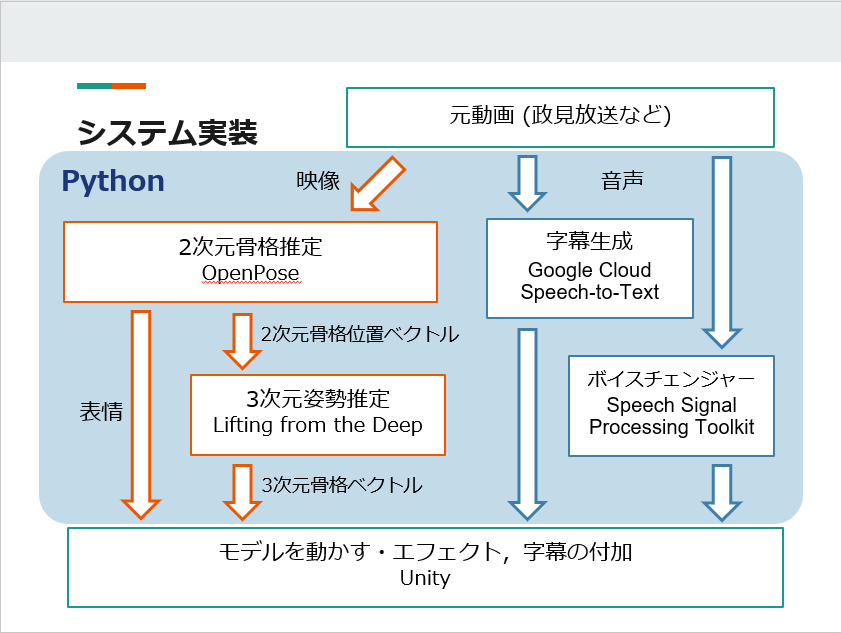
\includegraphics[width=7.5cm]{./fig/slide1.png}
				% \caption{}
				% \label{}
			\end{minipage}

			\begin{minipage}{0.50\hsize}
				\centering
				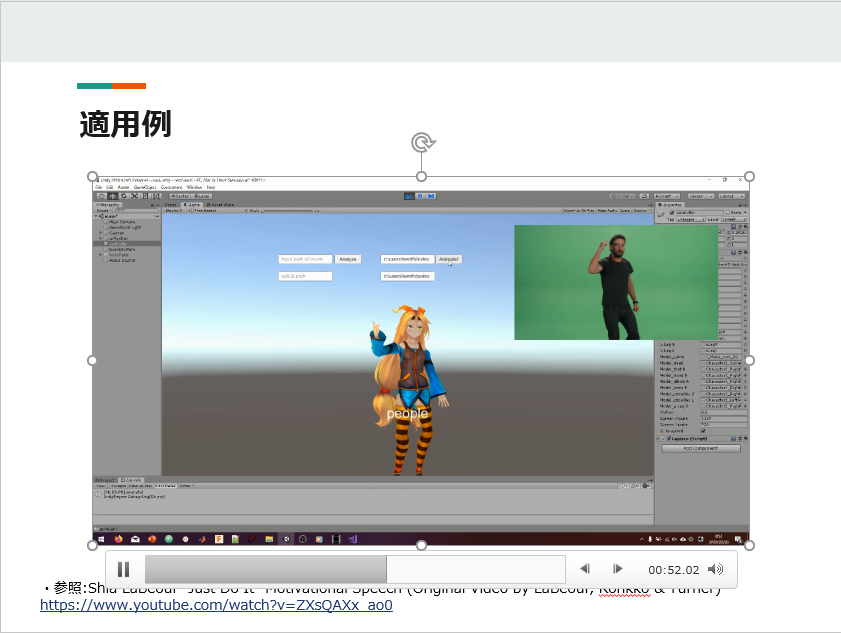
\includegraphics[width=7.5cm]{./fig/slide2.png}
				% \caption{}
				% \label{}
			\end{minipage}
		\end{tabular}
		% \label{}
	\end{center}
\end{figure}


\setcounter{section}{4}

\section{発表資料}

\subsection{課題設定発表での質疑応答一覧}

\begin{table}[H]
	\begin{tabular}{|l|l|} \hline
		{\bf 質問} & {\bf 回答} \\ \hline \hline
		骨格推定はできるか & Open Poseを用いることで可能 \\ \hline
		全員写すか, 1人にフォーカスするか & 1人にフォーカス\\ \hline
		各党でモデルを変えてはどうか & 公平性担保のためあまり変えない\\ \hline
		モデルは美少女のみか & はい\\ \hline
		可愛さのみで投票する恐れはないか & 各党でモデルに差異を付けない\\ \hline
		VTuber視聴割合のデータはあるか & 認知度のデータはある\\ \hline
		美少女でも討論は面白くないのでは & エフェクト等を工夫したい\\ \hline
		音声認識は難しいのでは & 字幕情報を使用する\\ \hline
		既存の政治解説VTuberとの差別化は & リアルタイムの用語解説を付加\\ \hline
		国会中継は動きがない & 動きのあるコンテンツを探す\\ \hline
		献血ポスターのように炎上する恐れ & 政治的中立性に則った上で関心を高めることが目的\\ \hline
	\end{tabular}
\end{table}

\subsection{中間発表での質疑応答一覧}

\begin{table}[H]
	\begin{tabular}{|l|l|} \hline
		{\bf 質問} & {\bf 回答} \\ \hline \hline
		国会中継から政見放送に変えたのか & 本システムを実装しやすいソースを選択した\\ \hline
		Open Poseの代替案(Pose Net等) & 検討する\\ \hline
		政見放送の権利問題, 著作権 & システムを政権に提供する形であれば問題なし\\ \hline
		他のものをソースにしてはどうか & エンタメ要素として活用できるため, 十分検討する\\ \hline
	\end{tabular}
\end{table}

\subsection{最終発表での質疑応答一覧}

\begin{table}[H]
	\begin{tabular}{|l|l|} \hline
		{\bf 質問} & {\bf 回答} \\ \hline \hline
		作成にあたり大変だった点はどこか & 開発言語が様々である各パートを組み合わせる点\\ \hline
	\end{tabular}
\end{table}

\end{document}
